Monitoring sentiment change in regards to releases can be done in bigger scale as well. In this section, instead of using tweets from several days before and after release, I have used the data collected weekly and analysed their relationship with number of releases per month. In the Figure \ref{fig:ReleasesSentiment3} are plotted sentiment difference from the average and the release count per month (red line represents sentiment while green stands for release count).

\begin{figure}[H]%
    \centering
    \subfloat[EmberJS]{{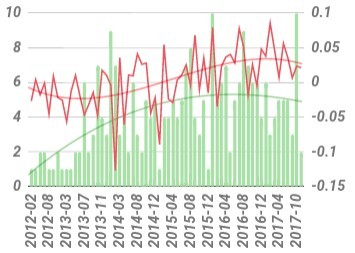
\includegraphics[width=5.5cm, height=4cm]{EmberReleasesSentiment.jpg} }}%
    \qquad
    \subfloat[Laravel]{{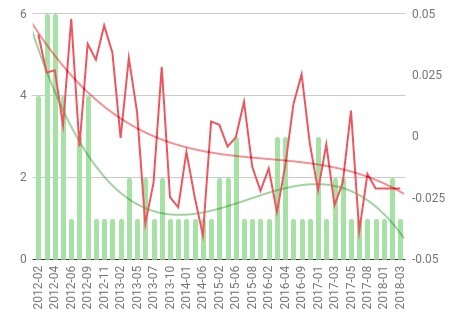
\includegraphics[width=5.5cm, height=4cm]{LaravelReleasesSentiment.jpg} }}%
    \label{fig:ReleasesSentiment1}%
\end{figure}


\begin{figure}[H]%
    \centering
    \subfloat[NodeJS]
    {{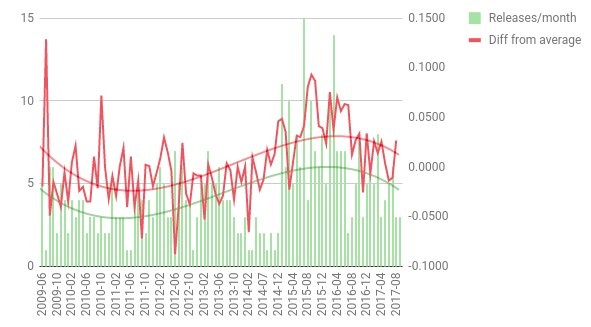
\includegraphics[width=5.5cm, height=4cm]{NodeReleasesSentiment.jpg} }}%
    \qquad
    \subfloat[VueJS]{{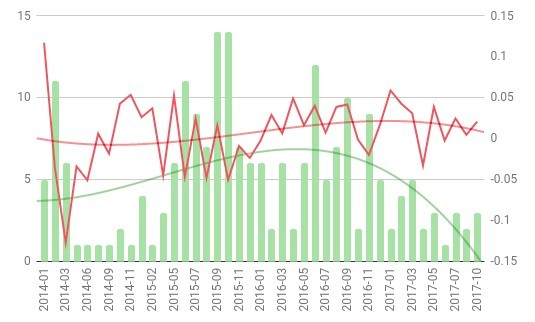
\includegraphics[width=5.5cm, height=4cm]{VueReleasesSentiment.jpg} }}%
    \label{fig:ReleasesSentiment2}%
\end{figure}


\begin{figure}[H]%
    \centering
    \subfloat[CakePhp]{{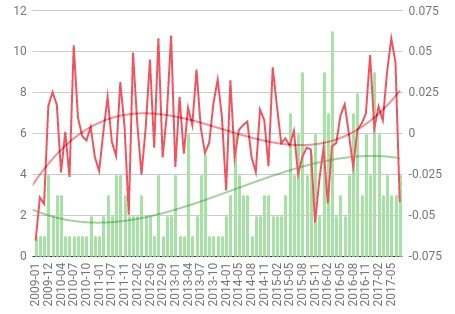
\includegraphics[width=5.5cm, height=4cm]{CakeReleasesSentiment.jpg} }}%
    \qquad
    \subfloat[AngularJS]{{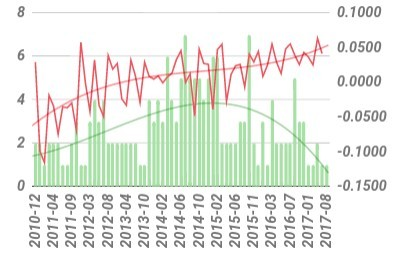
\includegraphics[width=5.5cm, height=4cm]{AngularReleasesSentiment.jpg} }}%
        \caption{Sentiment difference from average and release counts per month}
    \label{fig:ReleasesSentiment3}%
\end{figure}

Looking at linecharts gives some feeling and intuition whether and what type of relation there is. When working with time series, it often needs to be determined whether one series causes changes in another or vice versa and also measure this relationship quantitatively. To find this relationship, measuring a cross-correlation and finding a lag is one way how to do it. Lag represents the effect of change in one data series on the other several periods later. \\
\\
To ensure a cross-correlation calculation makes sense, first I have to determine, whether the data are stationary. A stationary time series is one whose properties do not depend on the time at which the series is observed\cite{hyndman5forecast}. More precisely, if y\textsubscript{t} is a stationary time series, then for all \textit{s}, the distribution of \textit{(y\textsubscript{t},…,y\textsubscript{t+s})} does not depend on \textit{t}.\\
\\
To determine whether my data are stationary, I have used the Dickey-Fuller test method of tseries package in R. Results can be seen in the Table \ref{table:stationarity_table_sentiment} and \ref{table:stationarity_table_release_count}.

\begin{table}[H]
\centering
\begin{tabular}{ |p{3cm}||p{3cm}|p{3cm}|  }
 \hline
 \multicolumn{3}{|c|}{Stationarity test of web frameworks sentiment data} \\
 \hline
 Framework & Dickey-Fuller & p-value\\
 \hline
 NodeJS   & -2.6775    &0.2964\\ \hline
 AngularJS &   -3.883  & 0.0199\\ \hline
 EmberJS & -4.0783 & 0.0199\\ \hline
 VueJS    &-3.438 & 0.0646\\ \hline
 CakePHP&   -3.480  & 0.04847\\ \hline
 Laravel& -2.57  & 0.3431\\ \hline
 Symfony& -4.3979  & 0.01\\ \hline
\end{tabular}
\caption{Stationarity test of sentiment}
\label{table:stationarity_table_sentiment}
\end{table}

\begin{table}[H]
\centering
\begin{tabular}{ |p{3cm}||p{3cm}|p{3cm}|  }
 \hline
 \multicolumn{3}{|c|}{Stationarity test of web frameworks release count} \\
 \hline
 Framework & Dickey-Fuller & p-value\\
 \hline
 NodeJS   & -2.896    &0.205\\ \hline
 AngularJS &   -2.547  & 0.353\\ \hline
 EmberJS & -3.297 & 0.0802\\ \hline
 VueJS    &-2.158 & 0.511\\ \hline
 CakePHP&   -3.224  & 0.08915\\ \hline
 Laravel& -2.368  & 0.425\\ \hline
 Symfony& -2.218  & 0.488\\ \hline
\end{tabular}
\caption{Stationarity test of release counts}
\label{table:stationarity_table_release_count}
\end{table}

As we can see, p-values are always higher than 0.05 what indicates non-stationarity of the data, therefore I cannot calculate the cross-correlation on them in this state. To transform non-stationary data into stationary, 2 approaches can be used. These are differencing and transforming.  I have taken data series and differenced the values in Listing \ref{lst:differencing}. I have executed both, seasonal differencing and stationary differencing.

\begin{lstlisting}[caption={Used differencing method in R},label={lst:differencing},language=R]
Differencing <- function(x,y)
{
 framework_x_seasdiff <- diff(x,differences=1)  # seasonal differencing
 framework_x_Stationary <- diff(framework_x_seasdiff, differences= 1)
 framework_y_seasdiff <- diff(y, differences=1)
 framework_y_Stationary <- diff(framework_y_seasdiff, differences= 1)
 return(list(framework_x_Stationary,framework_y_Stationary))
}
\end{lstlisting}
New differenced values do appear to be stationary in mean and variance, as the level and the variance of the series stays roughly constant over time. Sentiment for NodeJS before and after differencing can be seen in Figure \ref{fig:NodeJS_Sentiment_before_after}.
\begin{figure}[H]%
    \centering
    \subfloat[Before differencing]{{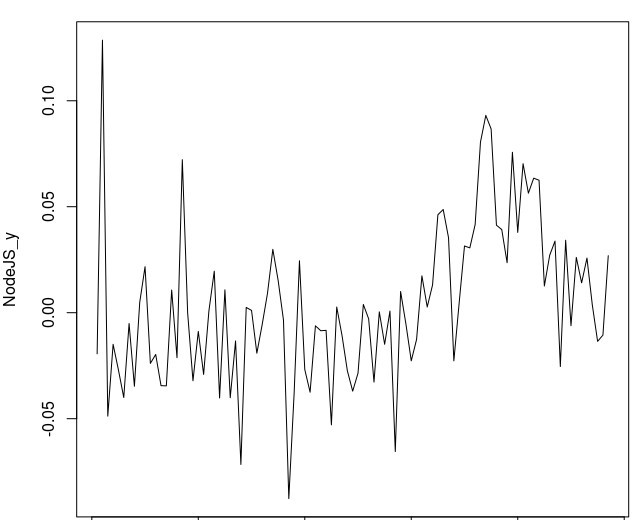
\includegraphics[width=5.5cm]{NodeJS_before.jpg} }}%
    \qquad
    \subfloat[After differencing]{{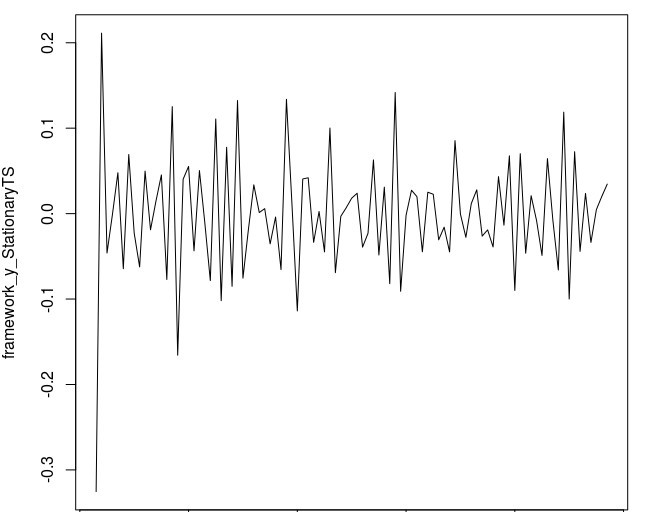
\includegraphics[width=5.5cm]{NodeJS_after.jpg} }}%
    \caption{NodeJS monthly sentiment values}%
    \label{fig:NodeJS_Sentiment_before_after}%
\end{figure}
Same procedure needed to be done with the "number of releases per month" data and afterwards. Then, cross-correlation could be executed. For this task I have used ccf method in R which implements Pearson's correlation calculation method. Results for all 7 OSS projects can be seen in Figure \ref{fig:highestCorrelationsPlotReleases}.\\
\begin{figure}[H]%
    \centering
	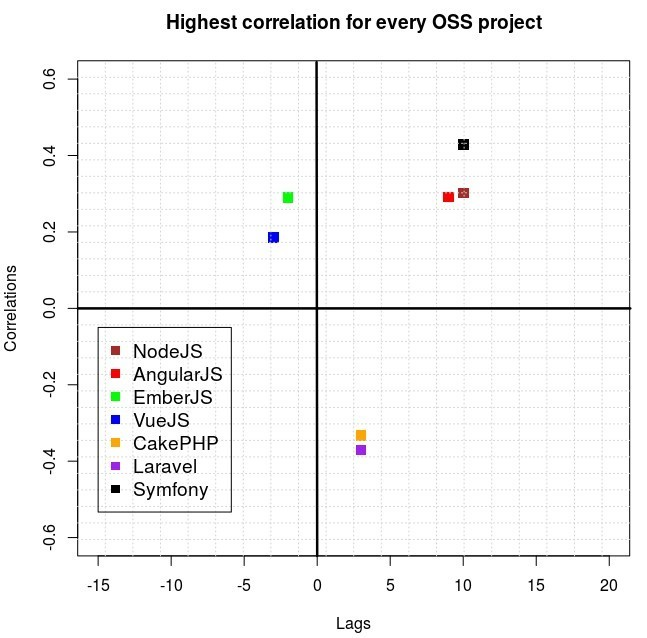
\includegraphics[width=8cm]{highestCorrelationsPlotReleases.jpg}
    \caption{Highest correlations for every OSS project}%
    \label{fig:highestCorrelationsPlotReleases}%
\end{figure}
I think there could be made a counter-point about whether the transformation to stationary data is really needed here, I have also included Figure \ref{fig:highestCorrelationsPlotReleases_nonStat} where are the results with the raw data.

\begin{figure}[H]%
    \centering
	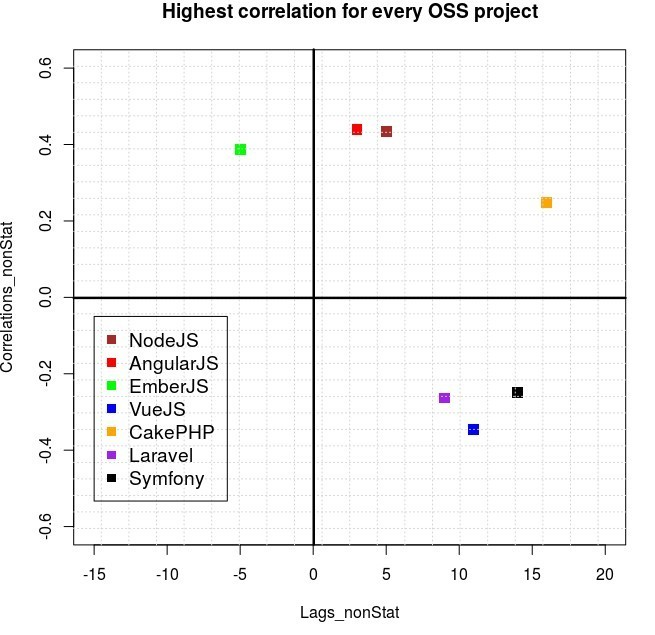
\includegraphics[width=8cm]{highestCorrelationsPlotReleases_nonStat.jpg}
    \caption{Highest correlations for every OSS project (non-stationary)}%
    \label{fig:highestCorrelationsPlotReleases_nonStat}%
\end{figure}

\paragraph{Results interpretation:}

Maximal project correlations happen to occupy 3 of 4 possible quadrants. Each quadrant represents a different relationship between number of releases and sentiment change. 3 out of 7 projects stayed in the same quadrant for both - stationary and non-stationary data.

\begin{itemize}
  \item \textbf{I. Quadrant}(Positive correlation + positive lag) - Increase of release count increases a sentiment in the upcoming months
  \item \textbf{II. Quadrant}(Positive correlation + negative lag) - Increase of sentiment increases a release count in the upcoming months
  \item \textbf{III. Quadrant}(Negative correlation + positive lag) - Increase of release count decreases a sentiment in the upcoming months
  \item \textbf{IV. Quadrant}(Negative correlation + Negative lag) - Increase of sentiment decreases a release count in the upcoming months
\end{itemize}

No project ended up in quadrant 3 so the potential result is that increasing release count definitely doesn't hinder project's sentiment. It can boost it but it is also not guaranteed.
